
\subsubsection{Initialization}

The initialization of the \ThermalRiderDesc\ starts with the implementation of the generic aspects of the Interaction Model (on which the \ThermalRiderDesc\ rides):
\begin{enumerate}
\item The Interaction Surface is created. 
\item The specific Interaction Model is initialized.  
\end{enumerate}
For specific information on these processes, see
the appropriate documents (
  \href{file:\JEODHOME/models/utils/surface\_model/docs/surface\_model.pdf}{Surface
  Model}\cite{dynenv:SURFACEMODEL} and,
  for example,
  \href{file:\JEODHOME/models/interactions/radiation\_pressure/docs/radiation\_pressure.pdf}{Radiation
  Pressure}\cite{dynenv:RADIATIONPRESSURE}).

\begin{enumerate}
\item  The initialization of the generic Interaction Surface has
little direct impact on this model, it creates the surface for later
population by an Interaction Model.
\item  The initialization of the specific Interaction Model must include the following
tasks:
\begin{enumerate}
\item The \textit{thermal.active} flag must be set (to be \textit{true} or \textit{false}).  If
it is set to false, the \ThermalRiderDesc\ will not be utilized.  The
rest of the initialization proceeds regardless of this flag setting;
this allows the user to switch the flag mid-simulation and still have
the \ThermalRiderDesc\ available immediately.
\item The initialization method for the specific instance of the
Interaction Surface (e.g. Radiation Surface) must be called.

The initialization routine for the surface calls the initialization routine for each facet in that surface, which in turn call the \textref{initialize}{ref:facetinitialize}
routine located in its attached ThermalFacetRider object.  

\end{enumerate}
\end{enumerate}



\subsubsection{Run-time}

The \ThermalRiderDesc\ functionality is first called from the Interaction Model with
which it is associated, as shown in figure \vref{fig:thermalflowchart1}.

The update function of the \ThermalRiderDesc\ comprises two sections (see
figure \vref{fig:thermalflowchart1a}).
\begin{enumerate}
\item The extent of the model is tested, to identify whether it is desirable to include additional thermal sources.  If so, the \textit{accumulate\_thermal\_sources} method is run from the Interaction Surface (see figure \vref{fig:thermalflowchart2}).

This surface version of this method in turn calls the
\textref{accumulate\_thermal\_sources}{ref:facetaccumulatethermalsources} 
method from the Thermal Facet Rider attached to each of the Interaction Facets.

This function (see figure \vref{fig:thermalflowchart3}) in turn simply adds the potential sources of energy for the given facet, and sets the default equilibrium condition that the power emitted and the power absorbed are equal.

\item  It can be useful to accumulate the power sources, even if there is no intent to monitor the temperature profile.  There is therefore another verification, that the user does intend that the temperature of the facets be variable.  If so, a call is made to the \textit{thermal\_integrator} from the Interaction Surface (see figure \vref{fig:thermalflowchart4}).

This function in turn 
calls the \textref{integrate}{ref:facetintegrate} method from the
Thermal Facet Riders attached to each of the Interaction Facets.

It is this method (see figure \vref{fig:thermalflowchart5}) that runs the 
RK4 integrator on the temperature.  The value of power emitted from the facet 
is re-calculated, obviously in light of the non-equilibrium conditions now being 
applied.  Finally, the Thermal Facet Rider on each facet stores the
integrated temperature (i.e. the temperature at the end of the next 
integration step) for later use.
\end{enumerate}



\begin{figure}[htp]
\begin{center}
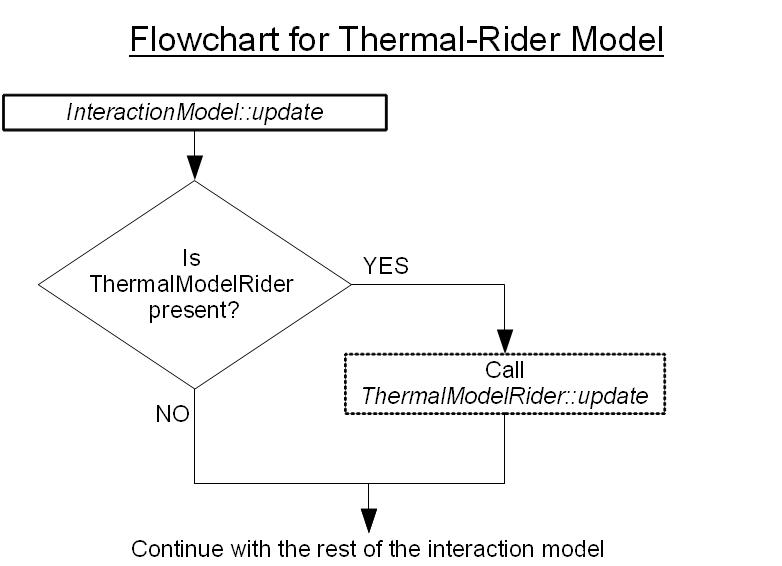
\includegraphics[height=3.8in]{figures/flow_chart_1.jpg}
\caption{Illustration of how the \ThermalRiderDesc\ is incorporated
into the simulation.}
\label{fig:thermalflowchart1}
\end{center}
\end{figure}

\begin{figure}[htp]
\begin{center}
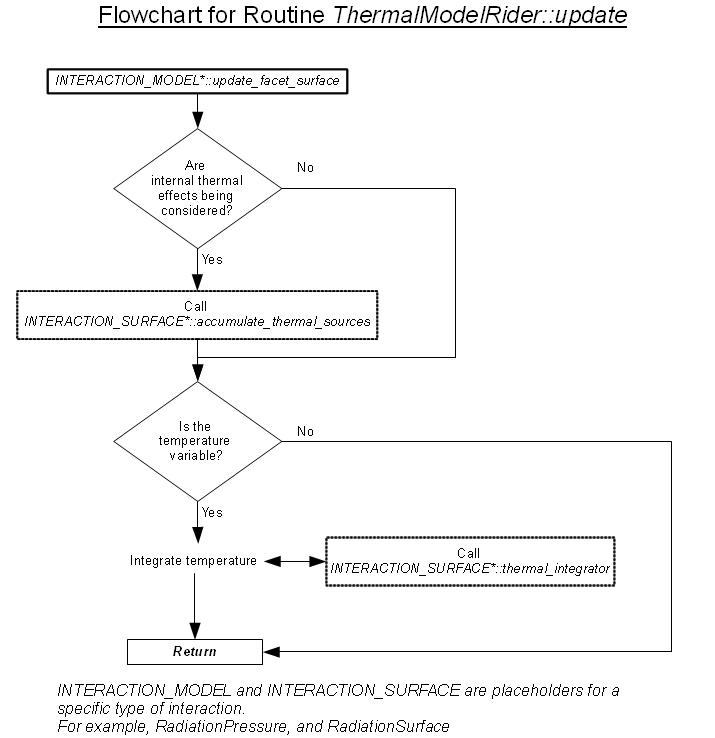
\includegraphics[height=7.2in]{figures/flow_chart_tmr_update.jpg}
\caption{The \ThermalRiderDesc\ controls the calls to the
interaction surface.}
\label{fig:thermalflowchart1a}
\end{center}
\end{figure}

\begin{figure}[htp]
\begin{center}
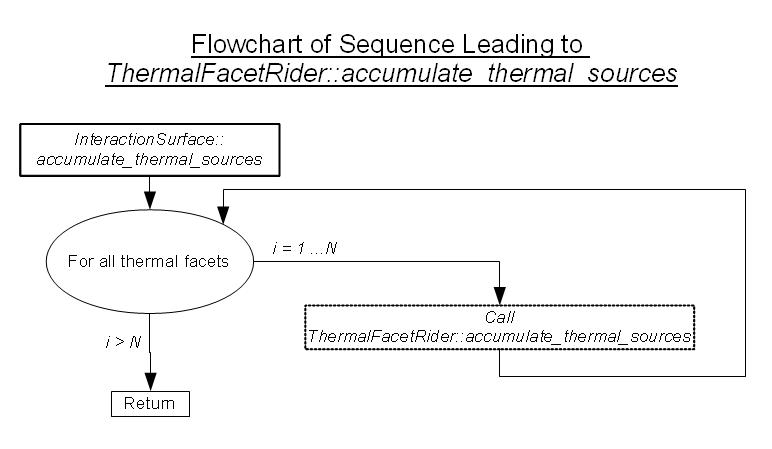
\includegraphics[height=3.9in]{figures/flow_chart_2.jpg}
\caption{The Interaction Surface controls the calls to each of the
interaction facets to independently accumulate the thermal sources on
that facet.}
\label{fig:thermalflowchart2}
\end{center}
\end{figure}

\begin{figure}[htp]
\begin{center}
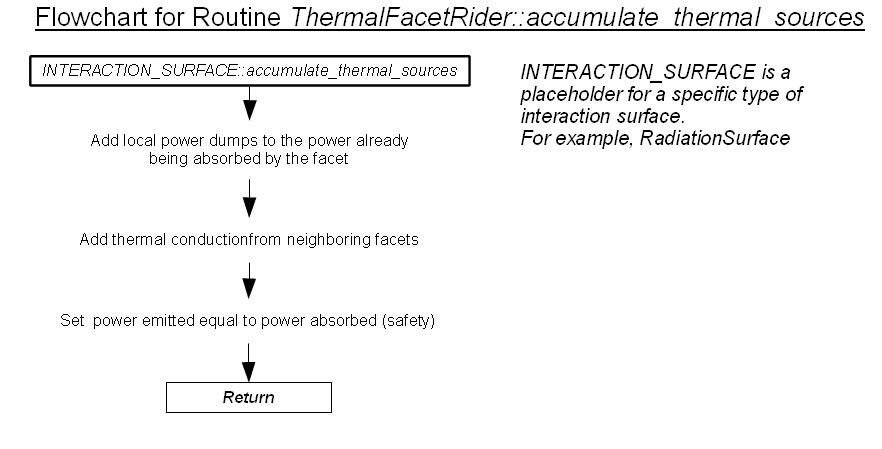
\includegraphics[height=3.4in]{figures/flow_chart_tfr_ats.jpg}
\caption{Each facet uses the functionality contained within its
thermal rider to collect (calculating where necessary) the thermal
sources being absorbed by that surface.}
\label{fig:thermalflowchart3}
\end{center}
\end{figure}

\begin{figure}[htp]
\begin{center}
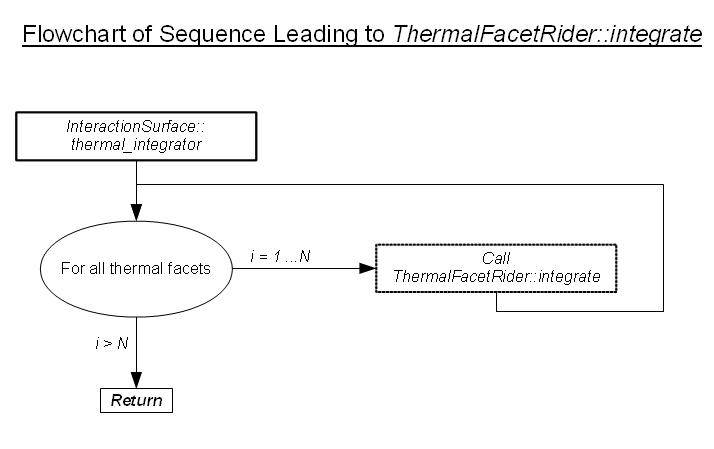
\includegraphics[height=4in]{figures/flow_chart_4.jpg}
\caption{The interaction surface controls the calls to each of the
interaction facets to independently integrate the rate of change of
temperature resulting from the accumulated thermal sources.} 
\label{fig:thermalflowchart4}
\end{center}
\end{figure}

\begin{figure}[htp]
\begin{center}
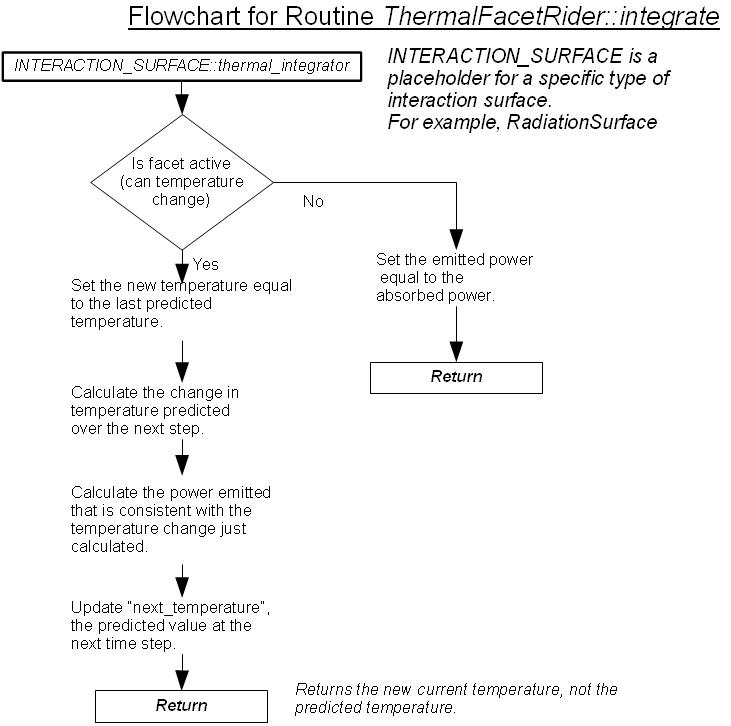
\includegraphics[height=6in]{figures/flow_chart_tfr_integrate.jpg}
\caption{Each facet uses the functionality contained within its 
thermal rider to integrate the temperature variation across one
integration step, and from that, determine the mean rate at which
thermal radiation was emitted.}
\label{fig:thermalflowchart5}
\end{center}
\end{figure}

